%%%%%%%%%%%%%%%%%%%%%%%%%%%%%%%%%%%%%%%%%
% Journal Article
% LaTeX Template
% Version 1.4 (15/5/16)
%
% This template has been downloaded from:
% http://www.LaTeXTemplates.com
%
% Original author:
% Frits Wenneker (http://www.howtotex.com) with extensive modifications by
% Vel (vel@LaTeXTemplates.com)
%
% License:
% CC BY-NC-SA 3.0 (http://creativecommons.org/licenses/by-nc-sa/3.0/)
%
%%%%%%%%%%%%%%%%%%%%%%%%%%%%%%%%%%%%%%%%%

%----------------------------------------------------------------------------------------
%	PACKAGES AND OTHER DOCUMENT CONFIGURATIONS
%----------------------------------------------------------------------------------------

\documentclass[twoside,twocolumn]{article}

\usepackage{blindtext} % Package to generate dummy text throughout this template 

\usepackage[sc]{mathpazo} % Use the Palatino font
\usepackage[T1]{fontenc} % Use 8-bit encoding that has 256 glyphs
\linespread{1.05} % Line spacing - Palatino needs more space between lines
\usepackage{microtype} % Slightly tweak font spacing for aesthetics

\usepackage[english]{babel} % Language hyphenation and typographical rules

\usepackage[hmarginratio=1:1,top=32mm,columnsep=20pt]{geometry} % Document margins
\usepackage[hang, small,labelfont=bf,up,textfont=it,up]{caption} % Custom captions under/above floats in tables or figures
\usepackage{booktabs} % Horizontal rules in tables

\usepackage{lettrine} % The lettrine is the first enlarged letter at the beginning of the text

\usepackage{enumitem} % Customized lists
\setlist[itemize]{noitemsep} % Make itemize lists more compact

\usepackage{abstract} % Allows abstract customization
\renewcommand{\abstractnamefont}{\normalfont\bfseries} % Set the "Abstract" text to bold
\renewcommand{\abstracttextfont}{\normalfont\small\itshape} % Set the abstract itself to small italic text

\usepackage{titlesec} % Allows customization of titles
\renewcommand\thesection{\Roman{section}} % Roman numerals for the sections
\renewcommand\thesubsection{\roman{subsection}} % roman numerals for subsections
\titleformat{\section}[block]{\large\scshape\centering}{\thesection.}{1em}{} % Change the look of the section titles
\titleformat{\subsection}[block]{\large}{\thesubsection.}{1em}{} % Change the look of the section titles

\usepackage{fancyhdr} % Headers and footers
\pagestyle{fancy} % All pages have headers and footers
\fancyhead{} % Blank out the default header
\fancyfoot{} % Blank out the default footer
\fancyhead[C]{Running title $\bullet$ May 2016 $\bullet$ Vol. XXI, No. 1} % Custom header text
\fancyfoot[RO,LE]{\thepage} % Custom footer text

\usepackage{titling} % Customizing the title section

\usepackage{hyperref} % For hyperlinks in the PDF

\usepackage{graphicx}

%----------------------------------------------------------------------------------------
%	TITLE SECTION
%----------------------------------------------------------------------------------------

\setlength{\droptitle}{-4\baselineskip} % Move the title up

\pretitle{\begin{center}\Huge\bfseries} % Article title formatting
\posttitle{\end{center}} % Article title closing formatting
\title{Article Title} % Article title
\author{%
\textsc{Frederik Vincent Primdahl} \textsc{Mikael Steenberg Pasovski} \and \textsc{Andreas Peter Brodersen} \textsc{Andreas Wede Gustavsen} \\[1ex] % Your name
\normalsize Copenhagen School of Design and Technology \\ % Your institution
%\and % Uncomment if 2 authors are required, duplicate these 4 lines if more
%\textsc{Jane Smith}\thanks{Corresponding author} \\[1ex] % Second author's name
%\normalsize University of Utah \\ % Second author's institution
%\normalsize \href{mailto:jane@smith.com}{jane@smith.com} % Second author's email address
}
\date{\today} % Leave empty to omit a date
\renewcommand{\maketitlehookd}{%
\begin{abstract}
\noindent \blindtext % Dummy abstract text - replace \blindtext with your abstract text
\end{abstract}
}

%----------------------------------------------------------------------------------------

\begin{document}

% Print the title
\maketitle

%----------------------------------------------------------------------------------------
%	ARTICLE CONTENTS
%----------------------------------------------------------------------------------------

\section{Introduction}
In the globalized economy of today, consumers are presented with a range of products to choose from when shopping. This can present some difficulty, as quality of the product is not always clear from its presentation. The customer review seeks to solve this by providing feedback on the purchase. Still, determining the value of a review can be difficult, as reviews can be misleading or provide little information.

Voting systems are often set in place to identify helpful reviews, and help consumers circumvent this issue, yet these reviews still get lost in the sheer number of unlabeled reviews. Our machine learning model aims to further filter reviews mainly by analyzing use of words, verbosity, among other aspects, to discover what makes a review helpful.

%------------------------------------------------
\section{Problem Formulation}

The main focus of this paper is to analyze Amazon review data across different categories and answer the question: “What makes an Amazon product review helpful?” through the use of classification models. In addition, answering “can you tell the helpfulness of a review based on name?”, “how does year affect the sentiment of the review?”

%------------------------------------------------
\section{Methods}

\subsection{Data exploration}

With the cleaned up dataset and the research question in mind, columns with relevance are explored. To explore, we plot different columns of interest to identify any patterns in the data in connection to review helpfulness. We plot the distribution between reviews with votes and no votes.
\begin{figure}[h]
	\centering
	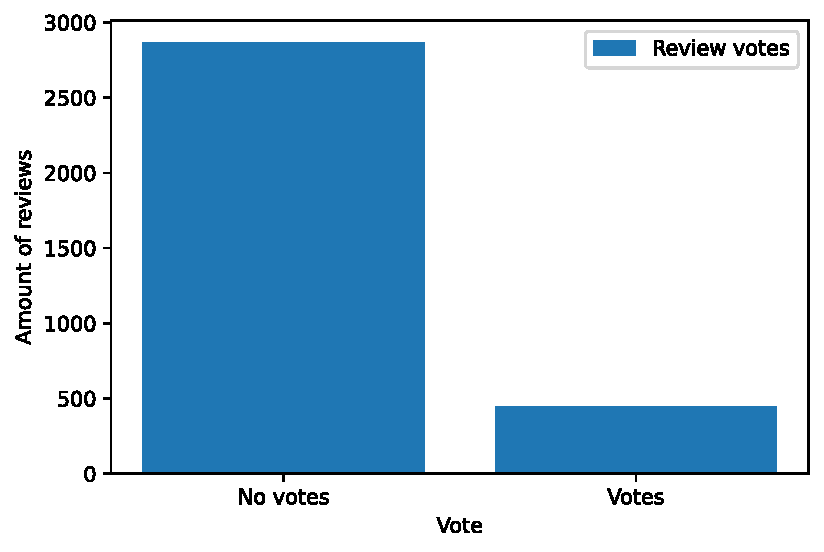
\includegraphics[width=0.5\textwidth]{img/no_votes_vs_votes.pdf}
	\caption{Upvote distribution}
	\label{fig:votes_distribution}
\end{figure}
As seen in \figurename{\ref{fig:votes_distribution}}, the distribution is very uneven in favor of reviews with no votes. This is relevant when evaluating performance metrics of our model, as it indicates that a statistic like Youden's Index might be useful to counteract random guessing. To get another perspective on review votes we plot the data into a heatmap in relation to ratings.
\begin{figure}[h]
	\centering
	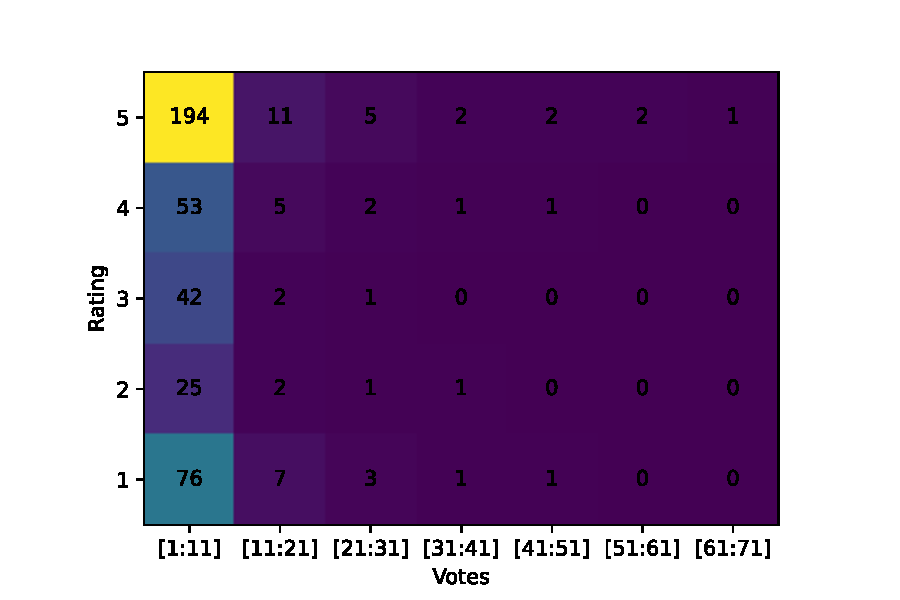
\includegraphics[width=0.5\textwidth]{img/rating_vote_heatmap_excluding_no_votes.pdf}
	\caption{Votes in relation to rating}
	\label{fig:rating_vote_heatmap}
\end{figure}
\figurename{\ref{fig:rating_vote_heatmap}} shows the ratings binned with the amount of votes. This heatmap only shows reviews with votes. The heatmap gives an indication of how votes combined with ratings are distributed in our dataset in a more specific way with the binned votes compared to \figurename{\ref{fig:votes_distribution}}.


%------------------------------------------------

\begin{figure*}[t]
	\centering% Do not use center environment, it adds additional vertical space

	\begin{center}
		\begin{tabular}{||c c c c c c||}
			\hline
			Count/TF-IDF & Classifier  & Train-set size & Parameters     & Time spend            & Youden's Index \\ [0.5ex]

			\hline\hline
			Count        & MLP         & 876.132        & LBFGS, 1x50    & 23min 5sec (i7 8700k) & 0.25646        \\

			\hline
			Count        & MLP         & 241.209        & Adam, 2x100    & 184min 24sec (M1 Air) & 0.23941        \\

			\hline
			Count        & MLP         & 107.302        & LBFGS, 1x100   & 2min 3sec (M1 Air)    & 0.23504        \\

			\hline
			Count        & LogisticReg & 107.302        & max iter=10000 & 17 sec (i7 6700k)     & 0.22513        \\

			\hline
			Count        & MLP         & 107302         & LBFGS, 1x50    & 2min 25sec(M1 Air)    & 0.22214        \\

			\hline
			Count        & SVC         & 107.302        & max iter=5000  & 58sec (M1 Air)        & 0.21384        \\

			\hline
			Count        & MLP         & 107.302        & Adam, 1x100    & 63min 2sec (M1 Air)   & 0.18065        \\

			\hline
			TF-IDF       & LogisticReg & 107.391        & max iter=10000 & 0.3sec (i7 6700k)     & 0.12344        \\

			\hline
			TF-IDF       & SVC         & 107.391        & max iter=5000  & 1.4sec (i7 6700k)     & 0.06107        \\


			\hline
		\end{tabular}
	\end{center}
	\caption{Model test runs}\label{Si_Results}
\end{figure*}

\section{Analysis}

\subsection{Data Preprocessing}
Initial data preparation was carried out on the whole dataset, dropping review time, image, style, ASIN, and reviewer id columns, as these were not needed. Unverified reviews were also filtered out, to avoid reviews from customers who did not purchase the product. Finally, null values were removed from the review text column.

As our input data mainly consists of unstructured text reviews, text normalization was done on the review text column to reduce randomness and reach a more uniform structure. This was done in accordance with common NLP data cleaning guidelines. Steps in this process involved removing non-word elements from the text – punctuation, symbols -, along with transforming each remaining word into lowercase. Because our model concerns itself with classification rather than sentiment, stop words like “not” did not provide any additional information to our model and were subsequently removed, as with other stop words contained in the NLTK “stopwords” library.

Each review was then tokenized into separate words using whitespace as a delimiter, as part of lemmatization to reduce morphological variation. Shortening some words to their root was thought important to improve model training efficiency. Lemmatization was chosen over stemming, as the accuracy of a lemmatizer in properly shortening words was more important than the speed of a stemmer.

As the next step of our data cleanup a column “voteSuccess” was added to the dataframe, calculating helpfulness of a review by dividing number of votes from the “votes”-column by quarters elapsed since the review was submitted. This was done to create a fairer indicator of helpfulness, since newer reviews would have had less time to accumulate helpfulness-votes and therefore appear less helpful.

For training our model, a numeric representation of our text corpus was needed for providing our models with input data. This was the final part of data preprocessing. Document-term matrices were created from two different vectorizations – Count and TF-IDF. Count vectorization parses a text corpus into a matrix based on the frequency of each term occurring in that corpus. This method was therefore the easiest way for us to present our data as something our classifiers could use. To discover if any less informative words not removed as part of our data cleanup were negatively impacting the performance of our model, we also opted for TF-IDF vectorization of our text data. TF-IDF favors unique terms appearing in documents higher, likely leading to a difference in model accuracy and precision metrics, and F1 scores.

\subsection{Model building}
To begin our model building LinearSVC was chosen as the initial classifier for our dataset. LinearSVC tries to classify our data into two groups, helpful and unhelpful since our problem is of a binary nature, and tries to find the optimal split between these two. Initially the model did not converge in time. We therefore tried different max iterations to see when the model would converge and avoid overfitting and find the best fit for classifying a review as helpful/unhelpful. Performance does take a hit as the data size increases, see \figurename{\ref{Si_Results}}.

After trying SVM as our first classifier, we wanted to try a neural network on the dataset. Both SVM and neural network seemed like a great place to start, since they can be used in most machine learning tasks and yield decent results.

We've used the Multi-layer Perceptron classifier with different amounts of hidden layers, nodes and solvers.

During our testing the performance scaled positively as the size of the dataset increased. The cost of using the Adam solver over the LBFGS is higher, increasing the fitting dramatically as the training set grows, which matches scikit-learn's documentation\cite{sklearn:MLPClassifier}.

Playing around with the nodes and layers got us to the ideal spot of 1 layer of 50 nodes, which scored highest on the Youden's Index % ###.

%------------------------------------------------

\section{Findings}

\subsection{Subsection One}

A statement requiring citation \cite{Figueredo:2009dg}.
\blindtext % Dummy text

\subsection{Subsection Two}

\blindtext % Dummy text

%------------------------------------------------
\section{Conclusion}


%----------------------------------------------------------------------------------------
%	REFERENCE LIST
%----------------------------------------------------------------------------------------

\begin{thebibliography}{99} % Bibliography - this is intentionally simple in this template

	\bibitem[Figueredo and Wolf, 2009]{Figueredo:2009dg}
	Figueredo, A.~J. and Wolf, P. S.~A. (2009).
	\newblock Assortative pairing and life history strategy - a cross-cultural
	study.

	\bibitem[scikit-learn MLPClassifier]{sklearn:MLPClassifier}
	\url{https://scikit-learn.org/stable/modules/generated/sklearn.neural_network.MLPClassifier.html} \newblock {\em Human Nature}, 20:317--330.

\end{thebibliography}

%----------------------------------------------------------------------------------------

\end{document}
